\id{МРНТИ 61.51.35,61.51.29}{https://doi.org/10.58805/kazutb.v.4.25-385}

\begin{articleheader}
\sectionwithauthors{Е.Г. Гилажов, Д.К. Кулбатыров, М.Д. Уразгалиева, А.Е. Законова, К.Р. Максот}{ЭФФЕКТИВНОСТИ ОКСИГЕНАТОВ НА ПОВЫШЕНИЕ ОКТАНОВОГО ЧИСЛА БЕНЗИНА С УСТАНОВКИ ЗАМЕДЛЕННОГО КОКСОВАНИЯ}

{\bfseries Е.Г.Гилажов, Д.К.Кулбатыров\textsuperscript{\envelope }, М.Д.Уразгалиева,
А.Е.Законова, К.Р.Максот}
\end{articleheader}

\begin{affiliation}
НАО «Атырауский университет нефти и газа имени С.Утебаева», Атырау,
Казахстан

\raggedright {\bfseries \textsuperscript{\envelope }}Корреспондент-автор: \href{mailto:dkkd@mail.ru}{\nolinkurl{dkkd@mail.ru}}
\end{affiliation}

Возрастание спроса на нефтегазовые продукты и их использование вызывает
различные серьезные экологические проблемы в мире. Основную часть
химического загрязнения окружающей среды составляют выхлопные газы
двигателей внутреннего сгорания. В результате физико-механических
процессов, происходящих в цилиндрах двигателя, выделяются комплексные
соединения, состоящие из нескольких токсичных компонентов. Современным
автомобилям требуется высокооктановое топливо с антидетонационными
свойствами, характеризующееся октановыми числами двигателя 92, 95 и 98.
Высокие антидетонационные характеристики достигаются либо путем глубокой
модификации бензинов с использованием процессов каталитического
крекинга, изомеризации, алкилирования, либо путем введения в топливо
специальных высокооктановых присадок. В настоящее время бензин занимает
одно из ведущих мест среди источников энергии первичного производства.
Потребность человечества в нем, в его высоком качестве, больше, чем в
любой другой фракции углеводородов. Поэтому к эксплуатационным свойствам
автомобильного бензина предъявляются очень высокие требования, и
проблема повышения качества бензина является одной из актуальных проблем
химической промышленности.

В представленной работе было испытано влияние оксигенатов
метил-\emph{трет}-бутилового эфира (МТБЭ) и диметилэтинилкарбинола
(ДМЭК) на повышение октанового числа бензина с установки замедленного
коксования (УЗК). Результаты исследования показали, что повышение
октанового числа бензина УЗК при добавлении ДМЭК и бинарной МТБЭ+ДМЭК
присадки выше, чем при добавлении МТБЭ. По результатам исследований
можно предположить, что, третичный ацетиленовый спирт -- ДМЭК можно
применить в качестве эффективной кислородсодержащей добавки для
автомобильных бензинов. Применение ДМЭК может расширить ресурсы
высокооктановых компонентов, снизить токсичность бензинов и отработанных
газов. Позволит увеличить выпуск высококачественного товарного бензина
для автомобильных двигателей.

{\bfseries Ключевые слова:} бензин установки замедленного коксования;
оксигенат; октановое число; диметилэтинилкарбинол; метил-трет-бутиловый
эфир; эффективность; детонация.

\begin{articleheader}
{\bfseries БАЯУ КОКСТЕУ ҚОНДЫРҒЫСЫ БЕНЗИННІҢ ОКТАН САНЫН АРТТЫРУҒА АРНАЛҒАН
ОКСИГЕНАТТАРДЫҢ ТИІМДІЛІГІ}

{\bfseries Е.Г.Гилажов, Д.К.Кулбатыров\textsuperscript{\envelope }, М.Д.Уразгалиева,
А.Е.Законова, К.Р.Мақсот}
\end{articleheader}

\begin{affiliation}
«С.Өтебаев атындағы Атырау мұнай және газ университеті» КЕАҚ, Атырау,
Қазақстан

е-mail: \href{mailto:dkkd@mail.ru}{\nolinkurl{dkkd@mail.ru}}
\end{affiliation}

Мұнай-газ өнімдеріне сұраныстың артуы және оларды пайдалану әлемдегі
әртүрлі экологиялық мәселелерді тудырады. Қоршаған ортаның химиялық
ластануының негізгі бөлігі ішкі жану қозғалтқыштарының газдары болып
табылады. Қозғалтқыш цилиндрлерінде болатын физика-механикалық
процестердің нәтижесінде бірнеше улы компоненттерден тұратын күрделі
қосылыстар бөлінеді. Қазіргі заманғы автомобильдерге қозғалтқыштарының
детонацияға қарсы қасиеттері бар октандық сандарымен сипатталатын 92, 95
және 98 жоғары октанды отын қажет. Детонацияға қарсы жоғары өнімділікке
каталитикалық крекинг, изомерлеу, алкилдеу процестерін қолдана отырып,
бензиндерді терең түрлендіру арқылы немесе отынға арнайы жоғары октанды
қоспаларды енгізу арқылы қол жеткізіледі. Қазіргі уақытта бензин
бастапқы өндірістің энергия көздері арасында жетекші орындардың бірін
алады. Адамзатқа бензиннің жоғары сапасына деген қажеттілігі,
көмірсутектердің басқа фракцияларына қарағанда көбірек. Сондықтан
автомобиль бензинінің пайдалану қасиеттеріне өте жоғары талаптар
қойылады және бензин сапасын арттыру мәселесі химия өнеркәсібінің өзекті
мәселелерінің бірі болып табылады.

Ұсынылған жұмыста метил-\emph{терт}-бутил эфирі (МТБЭ) және
диметилэтинилкарбинол (ДМЭК) оксигенаттарының баяу кокстеу қондырғысынан
(БКҚ) бензиннің октан санының жоғарылауына әсері сыналды. Зерттеу
нәтижелері ДМЭК және бинарлы МТБЭ+ДМЭК қосқанда БКҚ октан санының
жоғарылауы МТБЭ қосқанға қарағанда жоғары екенін көрсетті. Зерттеу
нәтижелері бойынша үшінші реттік ацетилен спирті -- ДМЭК автомобиль
бензиндері үшін тиімді оттегі бар қоспа ретінде қолданыла алады деп
болжауға болады. ДМЭК қолдану жоғары октанды компоненттердің ресурстарын
кеңейтіп, бензиндер мен пайдаланылған газдардың уыттылығын төмендетуі
мүмкін. Автомобиль қозғалтқыштары үшін жоғары сапалы тауарлық бензин
шығаруды ұлғайтуға мүмкіндік береді.

{\bfseries Түйін сөздер:~}баяу кокстеу қондырғысының бензині; оксигенат;
октан саны; диметилэтинилкарбинол; метил-трет-бутилды эфирі; тиімділік;
детонация.

\begin{articleheader}
{\bfseries EFFICIENCY OF OXYGENATES ON INCREASE OF OCTANE NUMBER OF
GASOLINE FROM DELAYED COKING UNIT}

{\bfseries Y.G.Gilazhov, D.K.Kulbatyrov\textsuperscript{\envelope } ,
M.D.Urazgalieva, A.E.Zakonova, K.R.Maksot}
\end{articleheader}

\begin{affiliation}
Non-profit JSC «Atyrau Oil and Gas University named after Safi
Utebayev», Atyrau, Kazakhstan,

е-mail: \href{mailto:dkkd@mail.ru}{\nolinkurl{dkkd@mail.ru}}
\end{affiliation}

The growth in demand and use of oil and gas products is the cause of a
number of serious environmental problems around the world. The main
source of chemical pollution in the environment is gases from internal
combustion engines. As a result of the physical and mechanical processes
that take place in the cylinders of the engine, complex compounds made
up of a number of toxic components are released. Modern cars require
high octane fuel with antidetonation properties, characterized by engine
octane numbers of 92, 95 and 98. High antidetonation properties are
achieved either by deep modification of petrol using catalytic cracking,
isomerization and alkylation processes, or by adding special high-octane
additives to the fuel. Today, gasoline is one of the most important
primary energy sources. More than any other hydrocarbon fraction,
humanity needs high quality gasoline. Therefore, very high demands are
placed on the operational properties of motor gasoline. The problem of
improving the quality of gasoline is one of the most pressing problems
of the chemical industry.

In the present work, the influence of methyl tert-butyl ether oxygenates
(MTBE) and dimethyl ethynyl carbinol (DMEC) on the increase of the
octane number of gasolines from a delayed coking unit (DCU) has been
tested. The results of the study showed that the increase in octane
number of DCU petrol when DMEС and binary MTBE+DMEС additives were added
was higher than that when MTBE was added. It can be concluded that
tertiary acetylene alcohol - DMEC can be used as an effective
oxygenating additive for automotive gasoline based on the research
results. The use of DMEC can expand the resources of high-octane
components, reduce the toxicity of gasoline and exhaust gases. It will
increase the output of high-quality commercial gasoline for automobile
engines.

{\bfseries Keywords:~} delayed coking unit gasoline, oxygenate, octane
number, dymethylethynylcarbinol, methyl tert-butyl ether, efficiency,
detonation.

\begin{multicols}{2}
{\bfseries Введение.} Повышение состояния экосистемы страны, в частности
соблюдение международных экологических требований в отношении токсичных
газов топлива и транспортных средств, окажет положительное влияние на
окружающую среду {[}1{]}. Возрастание спроса на нефтегазовые продукты и
их использование вызывает различные серьезные экологические проблемы в
мире. Основную часть химического загрязнения окружающей среды составляют
выхлопные газы двигателей внутреннего сгорания. В результате
физико-механических процессов, происходящих в цилиндрах двигателя,
выделяются комплексные соединения, состоящие из нескольких токсичных
компонентов {[}2,3{]}. В последнее время все больше обсуждается об этих
процессах. Основной причиной такого интереса является энергетический
кризис и рост цен на бензин. В то же время многие понимают, что выгоды
от добычи и продажи сырой нефти невелики. Представляется более выгодным
перерабатывать нефть на различные компоненты и продавать их. Основные
исследования в этой отрасли проводятся зарубежными учеными, в том числе
из США {[}4{]}.

Современным автомобилям требуется высокооктановое топливо с
антидетонационными свойствами, характеризующееся октановыми числами
двигателя 92, 95 и 98. Высокие антидетонационные характеристики
достигаются либо путем глубокой модификации бензинов с использованием
процессов каталитического крекинга, изомеризации, алкилирования, либо
путем введения в топливо специальных высокооктановых присадок. В
настоящей время бензин занимает одно из ведущих мест среди источников
энергии первичного производства. Потребность человечества в нем, в его
высоком качестве, больше, чем в любой другой фракции углеводородов.
Поэтому к эксплуатационным свойствам автомобильного бензина
предъявляются очень высокие требования, и проблема повышения качества
бензина является \emph{одной из актуальных проблем химической
промышленности.}

Основной мировой тенденцией в улучшении экологических и эксплуатационных
свойств автомобильных бензинов является использование
многофункциональных присадок, в основном оксигенатов --
кислородсодержащих веществ (спиртов, кетонов, эфиров и др.). Присутствие
кислорода в молекуле оксигенатного топлива позволяет снизить вредные
выбросы монооксида углерода на 30\%, а несгоревших углеводородов -- на
15\%. В США и ЕС содержание оксигенатов в бензине в количестве не менее
2\% по массовым долям в пересчете на кислород является обязательным. Уже
более 20 лет метил-\emph{трет}-бутиловый эфир (МТБЭ) является основным
оксигенатом, который способствует более полному сгоранию топлива и
повышает антидетонационные свойства бензина (октановое число по методике
исследования 115-135 единиц). Мировое производство МТБЭ из метанола и
изобутилена находится на уровне 20 миллионов тонн в год {[}5{]}. В
настоящее время из-за токсичности и опасности для окружающей среды он
уже запрещен во многих странах. Из-за экологической безопасности
применения МТБЭ, в качестве альтернативной добавки рассматриваются его
гомологи -- этиловый и бутиловый эфиры \emph{трет-}бутанола {[}6{]}. Для
уменьшения вредных выбросов выхлопных газов из двигателей внутреннего
сгорания, повышения сопротивления детонации топлива и использования
возобновляемого топлива, в базовый бензин добавляется много различных
кислородсодержащих присадок {[}7{]}. Исследовано влияние изобутанольной
добавки в метанол-бензиновое топливо немодифицированных двигателей с
искровым зажиганием. Показано что изобутанольные присадки являются
жизнеспособным вариантом для смешивания с существующим более низким
соотношением метанол-бензин для работы двигателя с искровым зажиганием в
качестве альтернативного топлива {[}8{]}. Установлено, что
арилбутилацетали обладают достаточно высоким октановым числом (ОЧ) (до
110 -- определенным исследовательским методом (ОЧИ)) и могут быть
перспективными добавками к автомобильным бензинам для повышения
детонационной стойкости, добавление 3 мас.\% арилбутилацеталя
увеличивает ОЧИ смеси н-гептан-изооктан в качестве модельного топлива и
базового топлива АИ-92-К5 на 1,0-1,2 и 0,1-0,4 пункта соответственно
{[}9{]}. Активно изучается применение других эфиров в качестве добавок к
бензину и дизельному топливу. На примере ряда моноэфиров гликолей
показано, что антидетонационная активность целлозольвов и карбитолов в
виде 1\%-ной добавки к прямогонной бензиновой фракции выше, чем у МТБЭ.
Это выражается в повышении октанового числа по исследовательскому методу
исходного бензина с 82,1 до 87,7-90,0 и 85,2 единиц, соответственно
{[}10{]}. \hl{}

С каждым годом критерии на качество используемого автомобильного топлива
становятся более требовательными. В связи с этим автоконцерны создают
двигатели внутреннего сгорания соответствующими этим критериям.
Использование низкокачественного автомобильного топлива ведет не только
к медленной езде, но и к поломке автомобиля в целом. В данном случае
рекомендуется использовать топливо, которое соотвествует условиям
эксплуатации. Достичь этого можно либо при использовании
высококачественного бензина, либо с при использовании специальных
средств, повышающих октановое число, так называемых присадок или
добавок.

Использование кислородсодержащих компонентов (оксигенатов), является
\emph{одним из перспективных способов получения высокооктанового
бензина.}

Как известно, мало изучены антидетонационные свойства третичных
ацетиленовых спиртов. Интересным фактом является то, что они содержат в
своей молекуле третичные алкильные радикалы, гидроксильные радикалы и
ацетиленовую непредельную группу, которая способна разрывать фронт
детонации. Исследование и разработка новых кислородсодержащих присадок
на основе третичных ацетиленовых спиртов, которые могут повысить
октановое число бензина, является важной и актуальной задачей.

Цель работы заключается в исследовании влияния таких оксигенатов, как
МТБЭ и диметилэтинилкарбинола (ДМЭК) на повышение октанового числа
бензина с установки замедленного коксования.

{\bfseries Материалы и методы.} Алифатический ацетиленовый спирт ДМЭК
получен методом конденсации ацетона (ГОСТ 2603-79 производства АО
«ЭКОС-1», ч.д.а.) и ацетилена (полученный из баллона промышленный по
ГОСТ 5457-75) в условиях модифицированной реакции Фаворского (рисунок
1).
\end{multicols}

\begin{figure}[H]
	\centering
	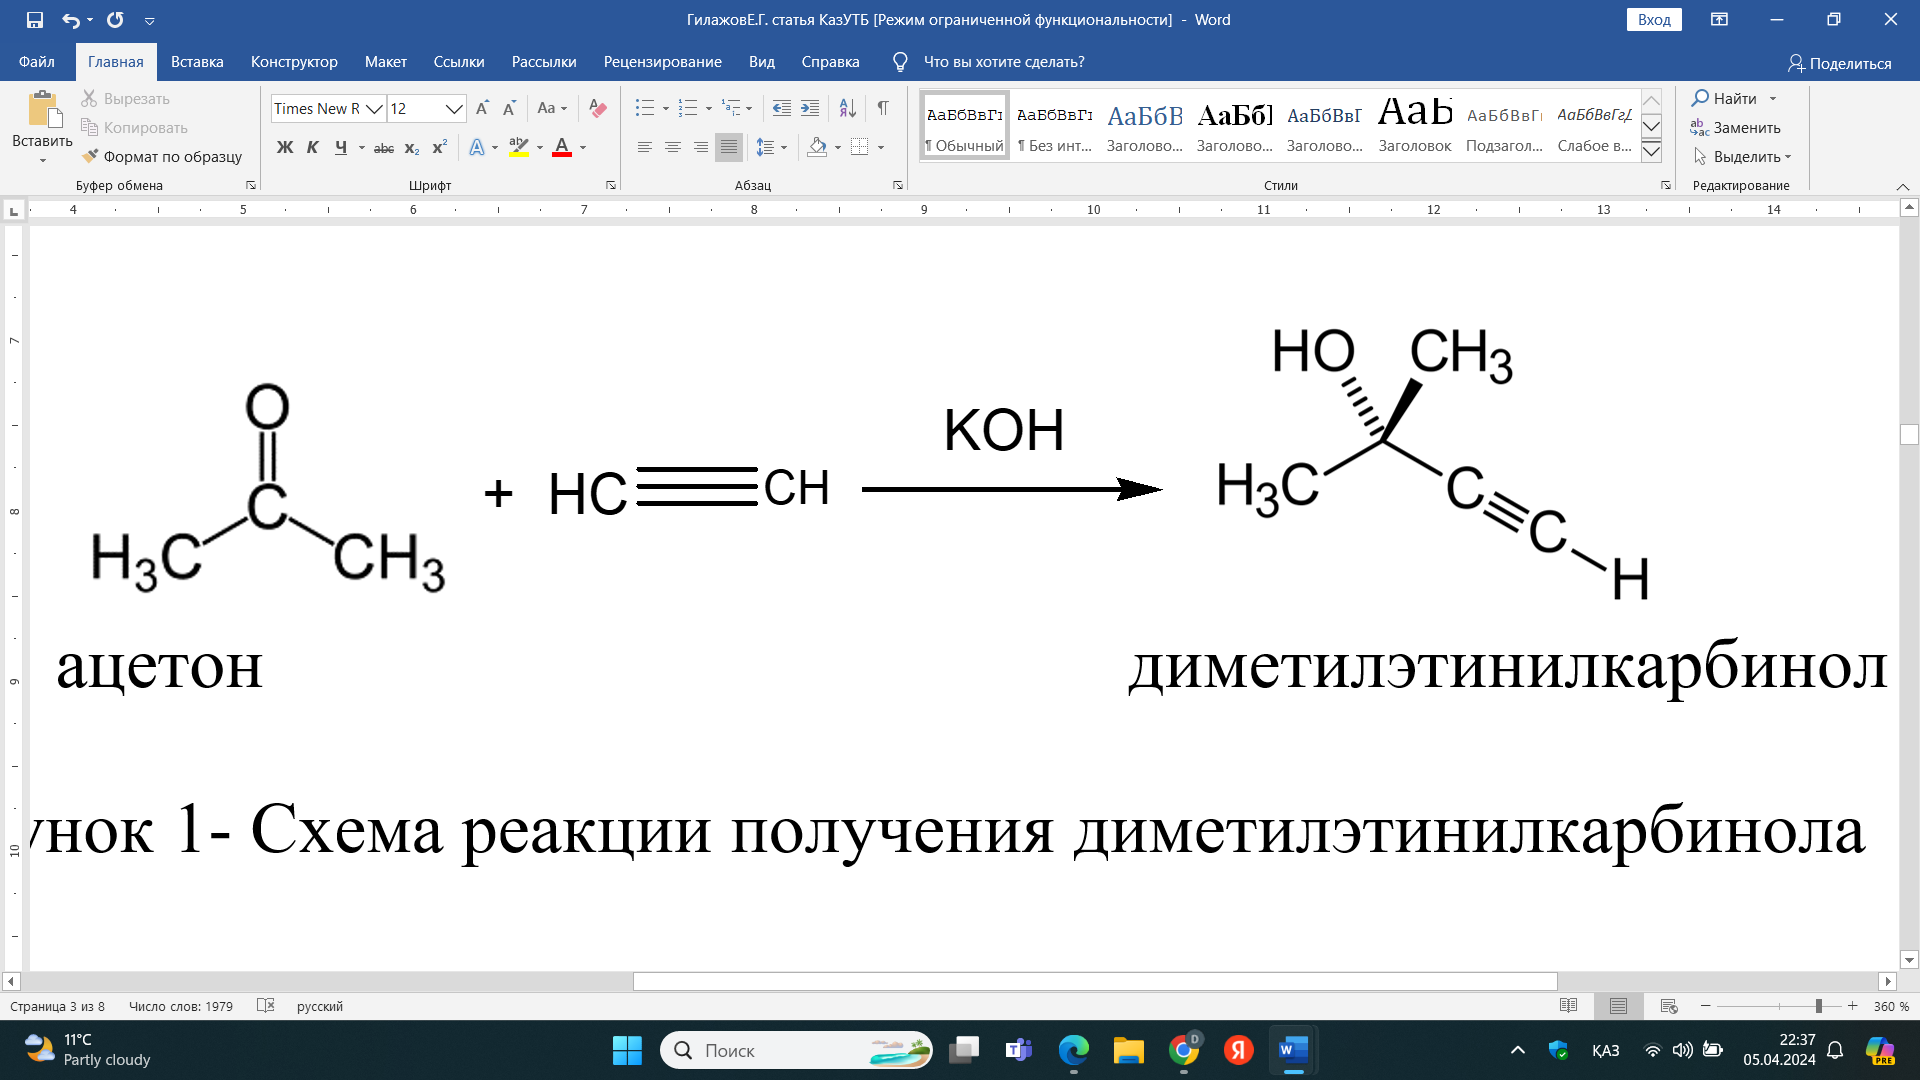
\includegraphics[width=0.6\textwidth]{media/chem/image13}
	\caption*{Рис. 1 - Схема реакции получения диметилэтинилкарбинола}
\end{figure}

Физико-химическое свойства синтезированного ДМЭК соответствует
литературным данным {[}11,12{]}.

\begin{table}[H]
\caption*{Таблица 1 -- Методы исследования и физико-химические свойства ДМЭК}
\centering
\begin{tabular}{|l|l|ll|p{0.1\textwidth}|}
\hline
\multirow{2}{*}{Характеристики} & \multirow{2}{*}{Методы исследования} & \multicolumn{2}{c|}{Литературные данные}           & Результаты исследования \\ \cline{3-5} 
                  &                  & \multicolumn{1}{l|}{{[}12{]}}    & {[}11{]}     &             \\ \hline
Состояние материи & визуальный       & \multicolumn{1}{l|}{жидкость}    & жидкость     & жидкость    \\ \hline
Плотность         & пикнометрический & \multicolumn{1}{l|}{0,86 г·см-3} & -            & 0,86 г·см-3 \\ \hline
Точка кипения     & ГОСТ 18995.6-73  & \multicolumn{1}{l|}{104 °C}      & 102 - 104 °C & 103-104 °C  \\ \hline
Показатель преломления          & рефрактрометричный                   & \multicolumn{1}{l|}{1,4209-1,4220} & 1,4208-1,4214 & 1,4209-1,4212           \\ \hline
\end{tabular}
\end{table}

\begin{table}[H]
\caption*{Таблица 2 -- Изменение октанового числа бензина УЗК, при добавлении МТБЭ}
\centering
\begin{tabular}{|l|r|rrr|rrr|}
\hline
\multirow{2}{*}{Бензин} &
  \multicolumn{1}{l|}{\multirow{2}{*}{\begin{tabular}[c]{@{}l@{}}МТБЭ\\   кол-во,\\   \%\end{tabular}}} &
  \multicolumn{3}{c|}{\begin{tabular}[c]{@{}l@{}}Октановое число, ОЧИ,\\   ГОСТ 8226-82\end{tabular}} &
  \multicolumn{3}{c|}{\begin{tabular}[c]{@{}l@{}}Октановое число, ОЧМ,\\   ГОСТ 511-82\end{tabular}} \\ \cline{3-8} 
 &
  \multicolumn{1}{l|}{} &
  \multicolumn{1}{l|}{без добавки} &
  \multicolumn{1}{l|}{с добавкой} &
  \multicolumn{1}{l|}{\begin{tabular}[c]{@{}l@{}}прирост\\   ОЧ\end{tabular}} &
  \multicolumn{1}{l|}{без добавки} &
  \multicolumn{1}{l|}{с добавкой} &
  \multicolumn{1}{l|}{\begin{tabular}[c]{@{}l@{}}прирост\\   ОЧ\end{tabular}} \\ \hline
\multirow{5}{*}{УЗК} &
  3 &
  \multicolumn{1}{r|}{\multirow{5}{*}{63,5}} &
  \multicolumn{1}{r|}{65} &
  1,5 &
  \multicolumn{1}{r|}{\multirow{5}{*}{62,1}} &
  \multicolumn{1}{r|}{63,1} &
  1 \\ \cline{2-2} \cline{4-5} \cline{7-8} 
 &
  5 &
  \multicolumn{1}{r|}{} &
  \multicolumn{1}{r|}{65,6} &
  2,1 &
  \multicolumn{1}{r|}{} &
  \multicolumn{1}{r|}{63,9} &
  1,8 \\ \cline{2-2} \cline{4-5} \cline{7-8} 
 &
  7 &
  \multicolumn{1}{r|}{} &
  \multicolumn{1}{r|}{66,7} &
  3,2 &
  \multicolumn{1}{r|}{} &
  \multicolumn{1}{r|}{65} &
  2,9 \\ \cline{2-2} \cline{4-5} \cline{7-8} 
 &
  11 &
  \multicolumn{1}{r|}{} &
  \multicolumn{1}{r|}{69} &
  5,5 &
  \multicolumn{1}{r|}{} &
  \multicolumn{1}{r|}{66,9} &
  4,8 \\ \cline{2-2} \cline{4-5} \cline{7-8} 
 &
  15 &
  \multicolumn{1}{r|}{} &
  \multicolumn{1}{r|}{70,3} &
  6,8 &
  \multicolumn{1}{r|}{} &
  \multicolumn{1}{r|}{68} &
  5,9 \\ \hline
\end{tabular}
\end{table}

\begin{table}[H]
\caption*{Таблица 3 - Изменение октанового числа бензина УЗК, при добавлении ДМЭК}
\centering
\begin{tabular}{|l|r|rrr|rrr|}
\hline
\multirow{2}{*}{Бензин} &
  \multicolumn{1}{l|}{\multirow{2}{*}{\begin{tabular}[c]{@{}l@{}}ДМЭК\\   кол-во,\\   \%\end{tabular}}} &
  \multicolumn{3}{c|}{\begin{tabular}[c]{@{}l@{}}Октановое число, ОЧИ,\\   ГОСТ 8226-82\end{tabular}} &
  \multicolumn{3}{c|}{\begin{tabular}[c]{@{}l@{}}Октановое число, ОЧМ,\\   ГОСТ 511-82\end{tabular}} \\ \cline{3-8} 
 &
  \multicolumn{1}{l|}{} &
  \multicolumn{1}{l|}{без добавки} &
  \multicolumn{1}{l|}{с добавкой} &
  \multicolumn{1}{l|}{\begin{tabular}[c]{@{}l@{}}прирост\\   ОЧ\end{tabular}} &
  \multicolumn{1}{l|}{без добавки} &
  \multicolumn{1}{l|}{с добавкой} &
  \multicolumn{1}{l|}{\begin{tabular}[c]{@{}l@{}}прирост\\   ОЧ\end{tabular}} \\ \hline
\multirow{5}{*}{УЗК} &
  3 &
  \multicolumn{1}{r|}{\multirow{5}{*}{63,5}} &
  \multicolumn{1}{r|}{68,3} &
  4,8 &
  \multicolumn{1}{r|}{\multirow{5}{*}{62,1}} &
  \multicolumn{1}{r|}{65,3} &
  3,2 \\ \cline{2-2} \cline{4-5} \cline{7-8} 
 &
  5 &
  \multicolumn{1}{r|}{} &
  \multicolumn{1}{r|}{69,3} &
  5,8 &
  \multicolumn{1}{r|}{} &
  \multicolumn{1}{r|}{65,7} &
  3,6 \\ \cline{2-2} \cline{4-5} \cline{7-8} 
 &
  7 &
  \multicolumn{1}{r|}{} &
  \multicolumn{1}{r|}{70,5} &
  7 &
  \multicolumn{1}{r|}{} &
  \multicolumn{1}{r|}{66,9} &
  4,8 \\ \cline{2-2} \cline{4-5} \cline{7-8} 
 &
  11 &
  \multicolumn{1}{r|}{} &
  \multicolumn{1}{r|}{73,8} &
  10,3 &
  \multicolumn{1}{r|}{} &
  \multicolumn{1}{r|}{70,2} &
  8,1 \\ \cline{2-2} \cline{4-5} \cline{7-8} 
 &
  15 &
  \multicolumn{1}{r|}{} &
  \multicolumn{1}{r|}{75,7} &
  12,2 &
  \multicolumn{1}{r|}{} &
  \multicolumn{1}{r|}{72,4} &
  10,3 \\ \hline
\end{tabular}
\end{table}

\begin{figure}[H]
	\centering
	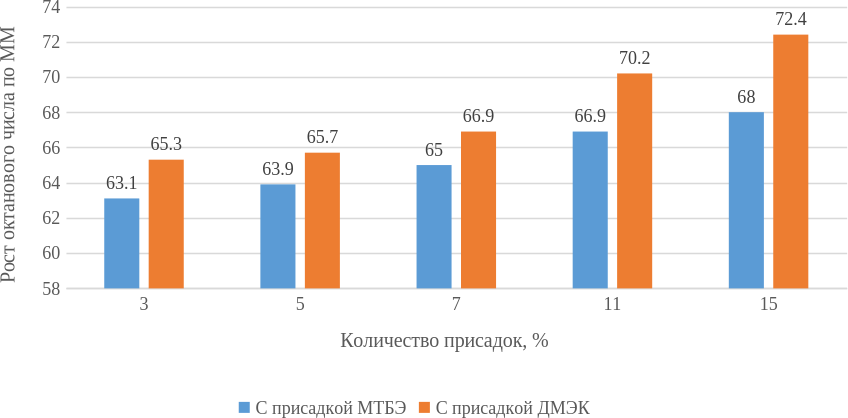
\includegraphics[width=0.8\textwidth]{media/chem/image98}
	\caption*{Рис. 2 -- Изменение октанового числа бензина УЗК при
добавлении МТБЭ и ДМЭК по ОЧИ}
\end{figure}

\begin{multicols}{2}
Реакция проведена под давлением в реакторе в присутствии
порошкообразного гидроксида калия в тетрагидрофуране. Исходные вещества
для синтеза ДМЭК применяли ацетон ТУ 2633-012-44493179-98 производства
АО «ЭКОС-1» и гидроксид калия ГОСТ 9285-78 производства ООО
«Сода-хлорат». Оксигенат МТБЭ производства «Компонент-реактив» с
содержанием основного вещества 99,9\%. Для исследования использовались
бензин с установки замедленного коксование (УЗК), производимого ТОО
«Атырауский нефтеперерабатывающий завод». Определение октанового числа
бензиновых композиций, содержащих предлагаемые добавки, проводилось
экспресс-методом на измерителе детонационной стойкости бензина на
октанометре SHATOX SX-100K (фирма изготовитель НПО «SHATOX», Институт
химических наук Сибирское отделение Российской академии наук (ИХН СО
РАН)). В качестве эталонов сравнения использованы параметры,
соответствующие ГОСТ Р 51866-2002 (ЕН 228-99) и ТУ
4215-002-60283547-2006. Результатами иследований взяты средние значения
трех повторностей испытаний.

{\bfseries Результаты и обсуждения.} Влияние оксигенатов МТБЭ и ДМЭК на
повышение октанового число бензина нами определялось по приросту
октанового числа бензина с УЗК производства ТОО «Атырауский
нефтеперерабатывающий завод». Эффективность кислородсодержащих присадок
(оксигенатов) в качестве высокооктановых компонентов исследовали при
введении их в бензин в концентрации от 3-х до15\% (масс.). В таблицах 2,
3 и на рисунках 2 и 3 представлены результаты добавки МТБЭ и ДМЭК по ОЧИ
и моторным методом (ОЧМ).
\end{multicols}

\begin{figure}[H]
	\centering
	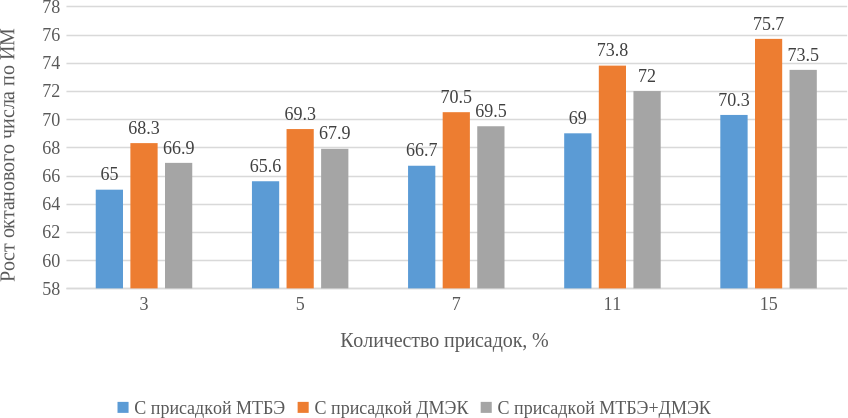
\includegraphics[width=0.8\textwidth]{media/chem/image99}
	\caption*{Рис. 3 -- Изменение октанового числа бензина УЗК при добавлении
МТБЭ и ДМЭК по ОЧМ}
\end{figure}

\begin{table}[H]
\caption*{Таблица 4 -- Изменение октанового числа бензина УЗК, при добавлении МТБЭ+ДМЭК = 1:1}
\centering
\resizebox{\textwidth}{!}{%
\begin{tabular}{|l|r|rrr|rrr|}
\hline
\multirow{2}{*}{Бензин} &
  \multicolumn{1}{l|}{\multirow{2}{*}{\begin{tabular}[c]{@{}l@{}}МТБЭ + ДМЭК=\\   1:1 кол-во, \%\end{tabular}}} &
  \multicolumn{3}{l|}{\begin{tabular}[c]{@{}l@{}}Октановое число, ОЧИ,\\   ГОСТ 8226-82\end{tabular}} &
  \multicolumn{3}{l|}{\begin{tabular}[c]{@{}l@{}}Октановое число, ОЧМ,\\   ГОСТ 511-82\end{tabular}} \\ \cline{3-8} 
 &
  \multicolumn{1}{l|}{} &
  \multicolumn{1}{l|}{без добавки} &
  \multicolumn{1}{l|}{с добавкой} &
  \multicolumn{1}{l|}{\begin{tabular}[c]{@{}l@{}}прирост\\   ОЧ\end{tabular}} &
  \multicolumn{1}{l|}{без добавки} &
  \multicolumn{1}{l|}{с добавкой} &
  \multicolumn{1}{l|}{\begin{tabular}[c]{@{}l@{}}прирост\\   ОЧ\end{tabular}} \\ \hline
\multirow{5}{*}{УЗК} &
  3 &
  \multicolumn{1}{r|}{\multirow{5}{*}{63,5}} &
  \multicolumn{1}{r|}{66,9} &
  3,4 &
  \multicolumn{1}{r|}{\multirow{5}{*}{62,1}} &
  \multicolumn{1}{r|}{65,1} &
  3 \\ \cline{2-2} \cline{4-5} \cline{7-8} 
 &
  5 &
  \multicolumn{1}{r|}{} &
  \multicolumn{1}{r|}{67,9} &
  4,4 &
  \multicolumn{1}{r|}{} &
  \multicolumn{1}{r|}{65,6} &
  3,5 \\ \cline{2-2} \cline{4-5} \cline{7-8} 
 &
  7 &
  \multicolumn{1}{r|}{} &
  \multicolumn{1}{r|}{69,5} &
  6 &
  \multicolumn{1}{r|}{} &
  \multicolumn{1}{r|}{66,9} &
  4,8 \\ \cline{2-2} \cline{4-5} \cline{7-8} 
 &
  11 &
  \multicolumn{1}{r|}{} &
  \multicolumn{1}{r|}{72} &
  8,5 &
  \multicolumn{1}{r|}{} &
  \multicolumn{1}{r|}{69} &
  6,9 \\ \cline{2-2} \cline{4-5} \cline{7-8} 
 &
  15 &
  \multicolumn{1}{r|}{} &
  \multicolumn{1}{r|}{73,5} &
  10 &
  \multicolumn{1}{r|}{} &
  \multicolumn{1}{r|}{70,6} &
  8,5 \\ \hline
\end{tabular}
}
\end{table}

\begin{multicols}{2}
Из рисунков 2 и 3 видно, что добавка ДМЭК повышает октановое число
бензина УЗК до 12,2 пунктов по ОЧИ и 10,3 пунктов по ОЧМ, а при
добавлении МТБЭ повышение октанового числа составляет по ОЧИ 6,8
пунктов, по ОЧМ 5,9 пунктов. Отсюда можно заметить, что эффективность
октаноповышающей добавки ДМЭК значительно выше, чем у МТБЭ.

Как известно из литературного поиска больший эффект достигается от
действия смеси при­садок вследствие проявления синергетического эф­фекта
{[}13-14{]}. Поэтому на втором этапе исследований была проверена
эффективность применения бинарных присадок, состоящих из ДМЭК и МТБЭ.
Октановые числа смешения присадок МТБЭ+ДМЭК = 1:1 в бензине УЗК
представлены в таблице 4 и на рисунках 4 и 5.
\end{multicols}

\begin{figure}[H]
	\centering
	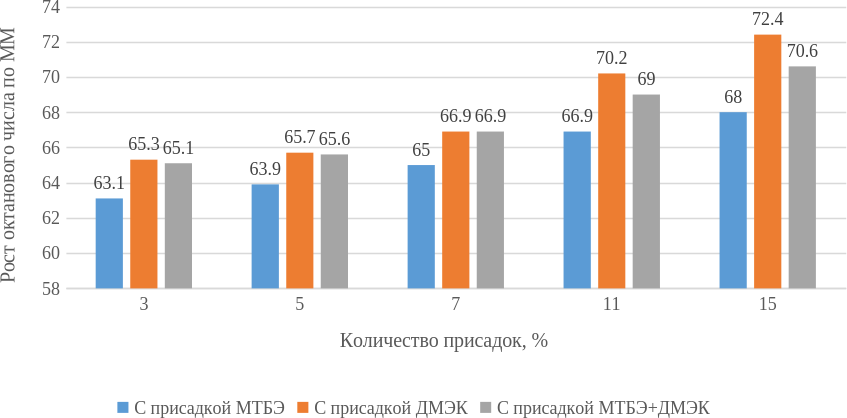
\includegraphics[width=0.8\textwidth]{media/chem/image100}
	\caption*{Рис. 4 - Изменение октанового числа бензина УЗК при добавлении
присадок МТБЭ+ДМЭК = 1:1 по ОЧИ}
\end{figure}

\begin{figure}[H]
	\centering
	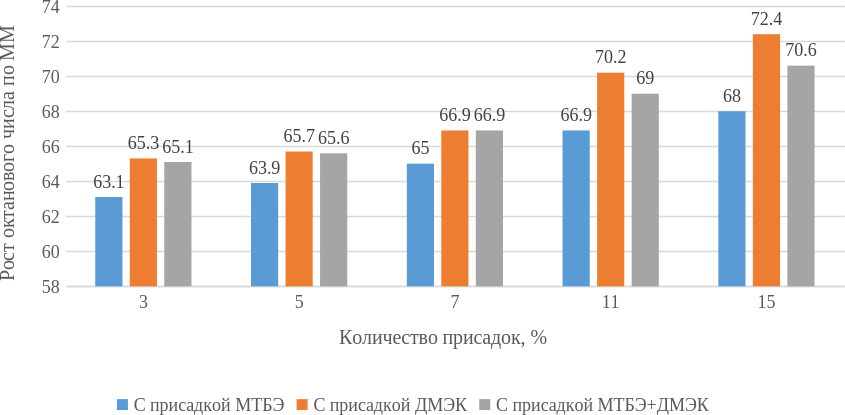
\includegraphics[width=0.8\textwidth]{media/chem/image101}
	\caption*{Рис. 5 - Изменение октанового числа бензина УЗК при добавлении
присадок МТБЭ+ДМЭК = 1:1 по ОЧМ}
\end{figure}

\begin{multicols}{2}
На рисунке 4 и 5 при исследовательском и моторном методах видно, что во
всех случаях повышение октанового числа за счет усиления
синергетического эффекта. При этом можно заметить, что, октановое число
бензина УЗК повышается при добавлении ДМЭК и бинарной присадки, чем при
добавлении МТБЭ.

{\bfseries Выводы.} Исследование влияния оксигенатов, как МТБЭ и ДМЭК на
повышение октанового числа бензина с установки замедленного коксования
показали, что повышение октанового числа бензина УЗК при добавлении ДМЭК
и бинарной присадки выше, чем при добавлении МТБЭ. По результатам
исследований можно предложить третичный ацетиленовый спирт -- ДМЭК как
кислородсодержащая добавка для автомобильных бензинов. Применение ДМЭК
может расширить ресурсы высокооктановых компонентов, снизить токсичность
бензинов и отработанных газов. Это позволит увеличить выпуск
высококачественного товарного бензина для автомобильных двигателей.

\emph{{\bfseries Финансирование}. Исследование была поддержана грантовым
финансированием Комитетом науки Министерства науки и высшего образования
Республики Казахстан. АР14148044/0222.}
\end{multicols}

\begin{center}
{\bfseries Литература}
\end{center}

\begin{references}
1.Махмудов M.Ж., Свайкосов С.О. Сравнение эффективности присадок в
повышении октанового числа бензина // Universum: технические науки:
электрон. научн. Журнал.- 2022.- № 6(99). -C. 24-29. URL:
\url{https://7universum.com/ru/tech/archive/item/14001}

2.Капустин В.М., Ершов М.А. и Хакимов Р.В. Автомобильные бензины с
высокооктановыми добавками, Москва: Российский государственный
университет нефти и газа (НИУ) имени И.М. Губкина, 2021. -160 с.

3.Makhmudov M.J., Svaykosov S.O., Abilov E.A. Method for reducing
aromatic hydrocarbons in \\composition of gasoline // Science and
Education in Karakalpakstan. -2021.- № 4.- С. 111-119

4.Дерюгина О.П., Мечик С.В., Трапезников Е.А. Процессы каталитического
риформинга и компаундирования как методы повышения октанового числа
бензинов, используемых в промышленных масштабах // Известия высших
учебных заведений. Нефть и газ. -2020.- № 3.- С. 89-99.
\url{https://doi.org/10.31660/0445-0108-2020-3-89-99}

5.Опарина Л.А., Колыванов Н.А., Гусарова Н.К., Сапрыгина В.Н.
Оксигенатные добавки к топливу на основе возобновляемого сырья //
Известия вузов. Прикладная химия и биотехнология. -2018. -Т. 8(1).-С.
19--34. \url{https://doi.org/10.21285/2227-2925-2018-8-1-19-34}

6.Ибрагимов Э.А., Абадзаде Х.И., Казимова А.Н., Ибрагимов Р.Г., Рустамов
М.И. Диизопропиловый эфир как перспективная оксигенатная добавка для
производства высокооктановых бензинов // Мир нефтепродуктов. Вестник
нефтяных компаний. 2014.- № 4. -С. 13-15.

7.Cakmak A., Ozcan H. Oxygenated Fuel Additives to Gasoline //
Politeknik dergisi. -2018. --Vol. 21(4).- P.831-840.
\url{https://doi.org/10.2339/politeknik.457956}

8.Hazim Sharudin, Nik Rosli Abdullah, G. Najafi, Rizalman Mamat, H.H.
Masjuki Investigation of the effects of iso-butanol additives on spark
ignition engine fuelled with methanol-gasoline blends // Аpplied thermal
engineering.- 2017.-Vol.114.-P.594-603

\url{https://doi.org/10.1016/j.applthermaleng.2016.12.017}

9.Колыванов, Н.А. Алкиларилацетали -- новый тип оксигенатных добавок к
моторным топливам / Л.А. Опарина, А.А. Ганина, С.Г. Дьячкова //
Нефтехимия. - 2020.- Т.60 (1).- С. 148 -153.
\\\href{https://doi.org/10.31857/S0028242120010104}{10.31857/S0028242120010104}

10.Хамидуллин Р.Ф., Харлампиди Х.Э., Пучкова Т.Л., Мельник А.Ю.,
Батрутдинова А.Р., Галиуллина М.М. Оксигенатные добавки к бензиновым
фракциям, повышающие октановые числа моторных топлив // Вестник
Казанского технологического университета.- 2014.- Т.17(21) -С. 295--300.

11.Щелкунов А.В., Васильева Р.Л., Кричевский Л.А. Синтез и взаимные
превращения монозамещенных ацетиленов. Алма-Ата: «Наука», 1975.- С.
44-45.

12.Academic dictionaries and encyclopedias. URL:
\href{https://de-academic.com/dic.nsf/dewiki/411193}{https://de-academic.com}. Дата обращения:
05.04.2024 г.

13.Danilov A.M. Research on Fuel Additives During 2011-2015.~//Chem
Technol Fuels Oils.~-2017. -Vol.53.-P.705-721.
\url{https://doi.org/10.1007/s10553-017-0853-z}

14.R. M. Nikulin, Kh. E. Kharlampidi, R. F. Khamidullin, A. V. Sitalo \&
F. A. Sharaf Synergistic Blend Based on Glycol Ethers as Antiknock
Additives to Motor Fuels // Chemistry and Technology of Fuels and
Oils.-2017.-Vol.52. - P.762-772.
\url{https://doi.org/10.1007/s10553-017-0771-0}
\end{references}

\begin{center}
{\bfseries References}
\end{center}

\begin{references}
1.Mahmudov M.Zh., Svajkosov S.O. Sravnenie jeffektivnosti prisadok v
povyshenii oktanovogo chisla benzina // Universum: tehnicheskie nauki:
jelektron. nauchn. Zhurnal.- 2022.- № 6(99). -C. 24-29. URL:
\url{https://7universum.com/ru/tech/archive/item/14001} {[}in Russian{]}

2.Kapustin V.M., Ershov M.A. i Hakimov R.V.
Avtomobil' nye benziny s vysokooktanovymi dobavkami,
Moskva: Rossijskij gosudarstvennyj universitet nefti i gaza (NIU) imeni
I.M. Gubkina, 2021. -160 s. {[}in Russian{]}

3.Makhmudov M.J., Svaykosov S.O., Abilov E.A. Method for reducing
aromatic hydrocarbons in \\composition of gasoline // Science and
Education in Karakalpakstan. -2021.- № 4.- С. 111-119

5.Oparina L.A., Kolyvanov N.A., Gusarova N.K., Saprygina V.N.
Oksigenatnye dobavki k toplivu na osnove vozobnovljaemogo
syr' ja // Izvestija vuzov. Prikladnaja himija i
biotehnologija. -2018. -T. 8(1).-S. 19--34.
https://doi.org/10.21285/2227-2925-2018-8-1-19-34

6.Ibragimov Je.A., Abadzade H.I., Kazimova A.N., Ibragimov R.G.,
Rustamov M.I. Diizopropilovyj jefir kak perspektivnaja oksigenatnaja
dobavka dlja proizvodstva vysokooktanovyh benzinov // Mir
\\nefteproduktov. Vestnik neftjanyh kompanij. 2014.- № 4. -S. 13-15.

7.Cakmak A., Ozcan H. Oxygenated Fuel Additives to Gasoline //
Politeknik dergisi. -2018. --Vol. 21(4).- P.831-840.
\url{https://doi.org/10.2339/politeknik.457956}

8.Hazim Sharudin, Nik Rosli Abdullah, G. Najafi, Rizalman Mamat, H.H.
Masjuki Investigation of the effects of iso-butanol additives on spark
ignition engine fuelled with methanol-gasoline blends // Аpplied thermal
engineering.- 2017.-Vol.114.-P.594-603

\url{https://doi.org/10.1016/j.applthermaleng.2016.12.017}

9.Kolyvanov, N.A. Alkilarilacetali -- novyj tip oksigenatnyh dobavok k
motornym toplivam / L.A. Oparina, A.A. Ganina, S.G.
D' jachkova // Neftehimija. - 2020.- T.60 (1).- S. 148
-153. \\https://doi.org/10.31857/S0028242120010104

10.Hamidullin R.F., Harlampidi H.Je., Puchkova T.L.,
Mel' nik A.Ju., Batrutdinova A.R., Galiullina M.M.
Oksigenatnye dobavki k benzinovym frakcijam, povyshajushhie oktanovye
chisla motornyh topliv // \\Vestnik Kazanskogo tehnologicheskogo
universiteta.- 2014.- T.17(21) -S. 295--300.

11.Shhelkunov A.V., Vasil' eva R.L., Krichevskij L.A.
Sintez i vzaimnye prevrashhenija \\monozameshhennyh acetilenov. Alma-Ata:
«Nauka», 1975.- S. 44-45.

12.Academic dictionaries and encyclopedias. URL:
\href{https://de-academic.com/dic.nsf/dewiki/411193}{https://de-academic.com}. Дата обращения:
05.04.2024 г.

13.Danilov A.M. Research on Fuel Additives During 2011-2015.~//Chem
Technol Fuels Oils.~-2017. -Vol.53.-P.705-721.
\url{https://doi.org/10.1007/s10553-017-0853-z}

14.R. M. Nikulin, Kh. E. Kharlampidi, R. F. Khamidullin, A. V. Sitalo \&
F. A. Sharaf Synergistic Blend Based on Glycol Ethers as Antiknock
Additives to Motor Fuels // Chemistry and Technology of Fuels and
Oils.-2017.-Vol.52. - P.762-772.
\url{https://doi.org/10.1007/s10553-017-0771-0}
\end{references}

\begin{authorinfo}
\hspace{1em}\emph{{\bfseries Сведения об авторе}}

Гилажов Е.Г.- доктор технических наук, профессор Института
нефтехимической инженерии и экологии, НАО «Атырауский университет нефти
и газа им. С. Утебаева», г. Атырау, Казахстан, e-mail: gilazhov@mail.ru;

Кулбатыров Д.К.- докторант Института нефтехимической инженерии и
экологии, НАО «Атырауский университет нефти и газа им. С. Утебаева», г.
Атырау, Казахстан, e-mail: dkkd@mail.ru;

Уразгалиева М.Д. -магистр, ведущий научный сотрудник Института
нефтехимической инженерии и экологии, НАО «Атырауский университет нефти
и газа им. С.Утебаева», г. Атырау, Казахстан, e-mail:
madina-uraz@mail.ru;

Законова А.Е.- преподователь Института нефтехимической инженерии и
экологии, НАО «Атырауский университет нефти и газа им. С. Утебаева», г.
Атырау, Казахстан, e-mail: z.aigerim\_17@mail.ru;

Максот К.Р.- магистрант Института нефтехимической инженерии и экологии,
НАО «Атырауский университет нефти и газа им. С. Утебаева», г. Атырау,
Казахстан, e-mail: kamilla.maksot@mail.ru

\hspace{1em}\emph{{\bfseries Information about the authors}}

Gilazhov Y.G. - Doctor of Technical Sciences, Professor of the Institute
of Petrochemical Engineering and Ecology, Non-profit JSC «Atyrau Oil and
Gas University named after Safi Utebayev», Atyrau, Kazakhstan, e-mail:
\href{mailto:gilazhov@mail.ru}{\nolinkurl{gilazhov@mail.ru}};

Kulbatyrov D.K. - Doctoral student at the Institute of Petrochemical
Engineering and Ecology, Non-profit JSC «Atyrau Oil and Gas University
named after Safi Utebayev», Atyrau, Kazakhstan, e-mail: dkkd@mail.ru;

Urazgalieva M.D.- Master' s degree, leading researcher of
the Institute of Petrochemical Engineering and Ecology, Non-profit JSC
«Atyrau Oil and Gas University named after Safi Utebayev», Atyrau,
Kazakhstan, e-mail: madina-uraz@mail.ru;

Zakonova A.E. - Lecturer at the Institute of Petrochemical Engineering
and Ecology, Non-profit JSC «Atyrau Oil and Gas University named after
Safi Utebayev», Atyrau, Kazakhstan, e-mail: z.aigerim\_17@mail.ru;

Maksot K.R.- Master' s student of the Institute of
Petrochemical Engineering and Ecology, Non-profit JSC «Atyrau Oil and
Gas University named after Safi Utebayev», Atyrau, Kazakhstan, e-mail:
kamilla.maksot@mail.ru
\end{authorinfo}
